% docs/slides/preamble.tex -- 五份 deck 共享
\documentclass[aspectratio=169,11pt]{beamer}

% ==== 中文与字体 ====
\usepackage[UTF8,fontset=none]{ctex}
\usepackage{fontspec}

\IfFontExistsTF{PingFang SC}{%
  \setCJKmainfont{PingFang SC}[BoldFont=PingFang SC,ItalicFont=PingFang SC,AutoFakeSlant=0.15]
  \setCJKsansfont{PingFang SC}[ItalicFont=PingFang SC,AutoFakeSlant=0.15]
  \setCJKmonofont{PingFang SC}
}{%
  \IfFontExistsTF{Source Han Sans SC}{%
    \setCJKmainfont{Source Han Sans SC}
    \setCJKsansfont{Source Han Sans SC}
  }{%
    \IfFontExistsTF{Noto Sans CJK SC}{%
      \setCJKmainfont{Noto Sans CJK SC}
      \setCJKsansfont{Noto Sans CJK SC}
    }{%
      \setCJKmainfont{Heiti SC}
      \setCJKsansfont{Heiti SC}
    }
  }
}

\IfFontExistsTF{Helvetica Neue}{\setmainfont{Helvetica Neue}}{%
  \IfFontExistsTF{Inter}{\setmainfont{Inter}}{}}
\IfFontExistsTF{JetBrains Mono}{\setmonofont{JetBrains Mono}[Scale=0.85]}%
  {\setmonofont{Menlo}[Scale=0.85]}

% ==== 颜色 ====
\usepackage{xcolor}
\definecolor{cMain}{HTML}{1F4E79}
\definecolor{cAccent}{HTML}{E07A1F}
\definecolor{cGray}{HTML}{595959}
\definecolor{cMute}{HTML}{F4F4F4}
\definecolor{cOK}{HTML}{2E7D32}
\definecolor{cBad}{HTML}{B23A3A}
\definecolor{cWarn}{HTML}{C8A300}

% ==== 主题 ====
\usepackage{tcolorbox}
\usetheme{metropolis}
\metroset{progressbar=frametitle,numbering=fraction,block=fill}
\setbeamercolor{frametitle}{bg=cMain,fg=white}
\setbeamercolor{progress bar}{fg=cAccent,bg=cMute}
\setbeamercolor{alerted text}{fg=cAccent}
\setbeamercolor{title}{fg=cMain}

% metropolis 默认尝试 Fira Sans，未安装时 fallback 到 Latin Modern Sans。
% 这里在主题加载后显式覆盖，强制使用 macOS 上一定存在的 Helvetica Neue，
% 跟中文 PingFang 风格一致；找不到则按顺序尝试 Inter / Arial。
\IfFontExistsTF{Helvetica Neue}{%
  \setsansfont{Helvetica Neue}%
}{%
  \IfFontExistsTF{Inter}{\setsansfont{Inter}}{%
    \IfFontExistsTF{Arial}{\setsansfont{Arial}}{}}%
}

% ==== TikZ ====
\usepackage{tikz}
\usetikzlibrary{positioning,arrows.meta,fit,shapes.geometric,calc,%
  decorations.pathmorphing,backgrounds}

\tikzset{
  node-box/.style={draw=cMain,thick,rounded corners=2pt,
    minimum height=8mm,minimum width=18mm,align=center,font=\small},
  node-state/.style={draw=cMain,thick,circle,minimum size=14mm,
    align=center,font=\small},
  node-ok/.style={draw=cOK,thick,fill=cOK!10},
  node-warn/.style={draw=cWarn,thick,fill=cWarn!15},
  node-bad/.style={draw=cBad,thick,fill=cBad!10},
  % 色盲友好的状态机三态：蓝 (正常/Closed) / 橙 (告警/Open) / 灰 (中间/HalfOpen)
  % 避免 red-green 二元区分，改用 hue + lightness 双通道。
  node-state-normal/.style={draw=cMain,thick,fill=cMain!12},
  node-state-alert/.style={draw=cAccent,thick,fill=cAccent!18},
  node-state-transition/.style={draw=cGray,thick,fill=cGray!18},
  arrow/.style={-{Stealth[length=2mm]},thick,draw=cMain},
  arrow-async/.style={-{Stealth[length=2mm]},thick,dashed,draw=cGray},
  arrow-bad/.style={-{Stealth[length=2mm]},thick,draw=cBad},
  arrow-alert/.style={-{Stealth[length=2mm]},thick,draw=cAccent},
  lifeline/.style={dashed,thick,draw=cGray},
}

% ==== 代码 ====
\usepackage{listings}
\lstdefinelanguage{Go}{
  morekeywords={break,case,chan,const,continue,default,defer,else,
    fallthrough,for,func,go,goto,if,import,interface,map,package,range,
    return,select,struct,switch,type,var,nil,true,false,iota},
  morekeywords=[2]{string,int,int64,uint,uint64,bool,byte,error,context},
  sensitive=true,
  morecomment=[l]//,morecomment=[s]{/*}{*/},
  morestring=[b]",morestring=[b]`,
}
\lstdefinelanguage{LuaRedis}{
  morekeywords={and,break,do,else,elseif,end,false,for,function,if,in,
    local,nil,not,or,repeat,return,then,true,until,while},
  morekeywords=[2]{redis,call,KEYS,ARGV,tonumber,HGET,HSET,GET,SET,
    DECR,DECRBY,INCR,INCRBY,EXPIRE,PEXPIRE,ZADD,ZCARD,ZREMRANGEBYSCORE,
    EVAL,EVALSHA},
  sensitive=true,
  morecomment=[l]{--},
  morestring=[b]",morestring=[b]',
}

\lstdefinestyle{base}{
  basicstyle=\ttfamily\scriptsize,
  numbers=left,numberstyle=\tiny\color{cGray},
  keywordstyle=\color{cMain}\bfseries,
  keywordstyle=[2]\color{cAccent},
  stringstyle=\color{cOK},
  commentstyle=\color{cGray}\itshape,
  backgroundcolor=\color{cMute},
  frame=single,framerule=0pt,
  showstringspaces=false,
  breaklines=true,
  tabsize=2,
  columns=fullflexible,
}
\lstset{style=base}

% ==== 三线表与附录页码 ====
\usepackage{booktabs}
\usepackage{appendixnumberbeamer}

% ==== 页脚来源标注 ====
\newcommand{\srcnote}[1]{{\color{cGray}\scriptsize\itshape #1}}

% 关键论点框
\newcommand{\keypoint}[1]{%
  \begin{tcolorbox}[colback=cMute,colframe=cMain,boxrule=0.5pt,arc=2pt]%
  #1\end{tcolorbox}}


\title{流量治理的业务依据}
\subtitle{gomall 各接口分级、阈值、SLO 与应急预案}
\author{gomall · 业务侧 deck}
\date{}

\begin{document}

\maketitle

\begin{frame}{今日大纲}
\tableofcontents
\end{frame}

% ============================================================
\section{为什么不能"一刀切"}
% ============================================================

\begin{frame}{deck 05 已经讲完技术，但有一个问题没回答}
\begin{itemize}
  \item deck 05 把令牌桶 / 滑动窗口 / 三态熔断器的\textbf{机制}讲清楚了。
  \item 真正决定生产是否平稳的，是另外两件事：
  \begin{itemize}
    \item \textbf{阈值要设多少} —— 100 RPS 还是 1000 RPS？
    \item \textbf{打开后用户看到什么} —— 直接 5xx 还是优雅降级？
  \end{itemize}
  \item 答这两个问题，必须先看业务，不能拍脑袋。
\end{itemize}
\srcnote{对应代码 routes/router.go:22, 96--119}
\end{frame}

\begin{frame}{gomall 在 router 里的三种治理姿态}
\begin{tikzpicture}[node distance=6mm and 10mm]
  \node[node-box] (cli) {Client};
  \node[node-box,right=of cli,node-warn] (gw) {全局 TokenBucket\\100 RPS / 200 burst};
  \node[node-box,right=of gw] (pay) {/paydown\\+CircuitBreaker};
  \node[node-box,below=of pay] (skill) {/skill\_product/skill\\+SlidingWindow 3/s};
  \node[node-box,above=of pay,node-ok] (rd) {/product/show\\无中间件};
  \draw[arrow] (cli) -- (gw);
  \draw[arrow] (gw) -- (pay);
  \draw[arrow] (gw) -- (skill);
  \draw[arrow] (gw) -- (rd);
\end{tikzpicture}
\vspace{2mm}
\srcnote{routes/router.go:22 全局；:96--103 paydown 熔断；:112--119 秒杀滑动窗口}
\end{frame}

% ============================================================
\section{接口分级：把 router 翻译成业务等级}
% ============================================================

\begin{frame}{第一步：把每个接口贴上业务标签}
\begin{tabular}{@{}llll@{}}
\toprule
等级 & 含义 & 限流策略 & 熔断策略 \\
\midrule
P0 核心交易 & 直接关联资金 & 宽松 & 必须有 \\
P1 核心读   & 影响转化       & 中等 & 可选 \\
P2 营销秒杀 & 反黑产强需求   & \textbf{激进} & 不需要 \\
P3 信息类   & 不在主路径     & 中等 & 不需要 \\
\bottomrule
\end{tabular}
\vspace{2mm}
\small 业务等级不是开发拍的，是产品 + 风控一起谈出来的。\\
gomall router 里能找到对应的中间件接入点（或缺失）。
\srcnote{原则参考阿里 Sentinel "核心业务" / "非核心业务" 切分理念}
\end{frame}

\begin{frame}{P0 核心交易 + P1 核心读}
\textbf{P0 \texttt{/orders/create}, \texttt{/paydown}}：直接关联资金。\textbf{宁可下游慢，不能上游 429}。
下单只挂 Idempotency，不挂 RateLimit；支付挂 CircuitBreaker，保护"第三方支付"这个外部依赖。

\vspace{2mm}
\textbf{P1 \texttt{/product/show}, \texttt{/orders/list}}：基线压测 62{,}226 / 58{,}406 RPS，已接近 \texttt{/ping} 上限。治理姿态：\textbf{靠缓存撑、不靠限流压}。深分页旧版 8.3 RPS / p95 16s 就是反面教材。
\srcnote{routes/router.go:39, 77, 78, 96--103；stressTest/REPORT.md 链路压测表}
\end{frame}

\begin{frame}{P2 营销秒杀：3/秒/用户 怎么来的}
\begin{itemize}
  \item 真实用户：点击 $\to$ 提交 $\to$ 等响应，最快 300--500ms 一次。
  \item 1 秒 3 次，留余量给"手抖双击"和"网络重试"，已经够宽。
  \item 超过 3 次/秒：八成是脚本或者多开浏览器。
  \item 阈值边界：
  \begin{itemize}
    \item 客服：通过 admin 接口直接补券，绕过秒杀链路。
    \item 真用户：基本不会触发。
    \item 黑产：第一波就被 70001 截断。
  \end{itemize}
\end{itemize}
\srcnote{routes/router.go:112--119 SlidingWindow Limit=3 Window=1s ByUser=true}
\end{frame}

\begin{frame}{P2 阈值校验：压测实测验证}
\textbf{场景}：30 VU $\times$ 15s 打 \texttt{/skill\_product/skill}，单 token，配置 3/秒/用户。

\vspace{2mm}
\begin{tabular}{@{}lrr@{}}
\toprule
指标 & 实测 & 业务期望 \\
\midrule
通过请求数 & 46  & 15s $\times$ 3 = 45 \\
被限流数   & 781{,}624 & 黑产应当被全部拦下 \\
误差       & 2.2\% & < 5\% 视为合格 \\
\bottomrule
\end{tabular}
\vspace{3mm}
\small "通过 46 次"≈"真用户最快也只能秒杀 45 次/15s"，业务侧合理。
\srcnote{stressTest/REPORT.md \S 5 限流中间件}
\end{frame}

\begin{frame}{P2 领券 + P3 信息类}
\textbf{P2 \texttt{/coupon/claim}}：Lua 单原子防超发，但\textbf{不防}"批量注册账号 $\times$ 每号 1 张"。
建议追加 \texttt{SlidingWindow\{Scope:"coupon", Limit:5, Window:1m, ByUser:true\}}：真用户 1min 领 5 张够用，万号脚本会卡在第 6 次。

\vspace{2mm}
\textbf{P3 \texttt{/carousels}、\texttt{/category/list}}：数据近不变，CDN / 长缓存为主。共享全局 TokenBucket 即可。SLO 99\% / p99 < 1s。
\srcnote{routes/router.go:43--44, 70}
\end{frame}

% ============================================================
\section{熔断打开后用户看到什么}
% ============================================================

\begin{frame}{熔断不是 5xx，是 200 + 业务码}
\begin{itemize}
  \item gomall 现在的实现：返回 200 + \texttt{status=70002}。
  \item 优点：app 端老网关吞不了 5xx，统一走业务码不会导致 crash。
  \item 缺点：监控不能简单按 4xx/5xx 算错误率，必须看业务 status。
  \item 业务文案：建议返回"支付服务繁忙，请稍后再试 (CB-OPEN)"。
\end{itemize}
\srcnote{middleware/circuitbreaker.go:58--65 当前返回的 JSON 结构}
\end{frame}

\begin{frame}{优雅降级的三个层次}
\begin{tikzpicture}[node distance=8mm and 12mm]
  \node[node-state,node-state-normal] (l1) {L1\\全功能};
  \node[node-state,node-state-transition,right=of l1] (l2) {L2\\先收单};
  \node[node-state,node-state-alert,right=of l2] (l3) {L3\\直接拒绝};
  \draw[arrow] (l1) -- node[above,font=\tiny]{依赖慢}(l2);
  \draw[arrow-alert] (l2) -- node[above,font=\tiny]{依赖挂} (l3);
\end{tikzpicture}
\vspace{2mm}
\begin{itemize}
  \item \textbf{L1}：正常调下游，正常返回。
  \item \textbf{L2}："先收单 / 异步扣款"：把请求记账到 outbox，下游恢复后补单。
  \item \textbf{L3}："服务暂时不可用"。
\end{itemize}
\small gomall 已有的 Outbox 模式（deck 04）天然支持 L2 兜底。
\srcnote{repository/cache/ratelimit.go:18--34；docs/slides/04-outbox-saga.tex 配套}
\end{frame}

\begin{frame}{熔断 + 重试 + 幂等的三角关系}
\begin{tikzpicture}[node distance=10mm and 16mm]
  \node[node-box] (cli) {客户端};
  \node[node-box,right=of cli,node-warn] (cb)  {CircuitBreaker};
  \node[node-box,right=of cb,node-ok] (id)  {Idempotency};
  \node[node-box,below=of id] (down) {Downstream};
  \draw[arrow]      (cli) -- (cb);
  \draw[arrow]      (cb)  -- (id);
  \draw[arrow]      (id)  -- (down);
  \draw[arrow-bad,bend left=30] (cb.south) to node[below,font=\tiny]{Open: 直接 70002} (cli.south);
\end{tikzpicture}
\vspace{2mm}
\begin{itemize}
  \item 客户端拿到 70002 $\to$ 触发\textbf{指数退避重试}。
  \item 重试必须带原 Idempotency-Key $\to$ 即使老请求其实成功了，也不会扣两次。
  \item 这是 router 里 paydown 同时挂 CircuitBreaker + Idempotency 的真正原因。
\end{itemize}
\srcnote{routes/router.go:96--103 paydown 中间件链}
\end{frame}

\begin{frame}[fragile]{Open 态：客户端拿到的 JSON}
\begin{lstlisting}[language=Go,firstnumber=57,
  caption={\srcnote{middleware/circuitbreaker.go:57--64}}]
if err := cb.allow(); err != nil {
    c.JSON(http.StatusOK, gin.H{
        "status": e.ErrCircuitOpen,          // 70002
        "msg":    e.GetMsg(e.ErrCircuitOpen),
        "data":   err.Error(),
    })
    c.Abort(); return
}
\end{lstlisting}
\small \textbf{业务侧约定}：\texttt{status=70002} = "请稍后重试"，\textbf{不是}订单失败。
\end{frame}

% ============================================================
\section{SLA / SLO：怎么给业务方一个数字}
% ============================================================

\begin{frame}{SLA / SLO / SLI 三个词}
\begin{tabular}{@{}lll@{}}
\toprule
术语 & 含义 & 谁负责 \\
\midrule
SLI & 实际测出来的指标 & 平台 / 监控 \\
SLO & 我们承诺的目标   & 平台 + 业务 \\
SLA & 不达标的赔付条款 & 法务 + 商务 \\
\bottomrule
\end{tabular}
\vspace{3mm}
\small 对 gomall 这个体量，更精准的说法是"内部 SLO"，对外不签 SLA。\\
开发同学常说的"SLA 99.95"严格意义是 SLO。
\srcnote{参考 Stripe / AWS 公开 SLA 文档结构}
\end{frame}

\begin{frame}{gomall 各业务等级的内部 SLO}
\begin{tabular}{@{}llll@{}}
\toprule
等级 & 接口举例 & 可用率 & 延迟 \\
\midrule
P0 交易 & /orders/create, /paydown      & \textbf{99.95\%} & p99 < 500ms \\
P1 读   & /product/show, /orders/list   & 99.9\%  & p99 < 200ms \\
P2 营销 & /skill\_product/skill         & 99\%    & p99 < 200ms \\
P3 信息 & /carousels, /category/list    & 99\%    & p99 < 1s    \\
\bottomrule
\end{tabular}
\vspace{3mm}
\small 可用率 99.95\% 全年宕机预算 4h22min；99\% 则有 87h。\\
P0 一年只能掉一个上午；P2 可以掉一整周晚高峰用于压测。
\srcnote{Stripe 公开过 90 天平均 5 个 9（99.999\%）的水平作为对照锚点}
\end{frame}

\begin{frame}{99.95\% 是怎么算出来的}
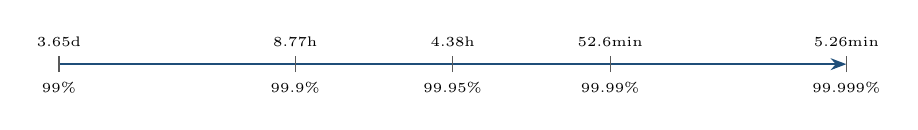
\begin{tikzpicture}
  \draw[arrow] (0,0) -- (10,0);
  \draw[cGray] (0,-0.1) -- (0,0.1); \node[font=\tiny,below] at (0,-0.1) {99\%};
  \draw[cGray] (3,-0.1) -- (3,0.1); \node[font=\tiny,below] at (3,-0.1) {99.9\%};
  \draw[cGray] (5,-0.1) -- (5,0.1); \node[font=\tiny,below] at (5,-0.1) {99.95\%};
  \draw[cGray] (7,-0.1) -- (7,0.1); \node[font=\tiny,below] at (7,-0.1) {99.99\%};
  \draw[cGray] (10,-0.1) -- (10,0.1); \node[font=\tiny,below] at (10,-0.1) {99.999\%};
  \node[font=\tiny,above] at (0,0.1) {3.65d};
  \node[font=\tiny,above] at (3,0.1) {8.77h};
  \node[font=\tiny,above] at (5,0.1) {4.38h};
  \node[font=\tiny,above] at (7,0.1) {52.6min};
  \node[font=\tiny,above] at (10,0.1) {5.26min};
\end{tikzpicture}
\vspace{4mm}
\small 每多一个 9，宕机预算砍 10 倍。
\begin{itemize}
  \item 99.95\% $\to$ 一年大概 4h22min 不可用，覆盖一次发版回滚没问题。
  \item 99.99\% 起，必须做\textbf{多可用区}、\textbf{热升级}，gomall 单机部署做不到。
\end{itemize}
\end{frame}

\begin{frame}{p99 < 500ms 在 gomall 的根据}
\begin{tabular}{@{}lrr@{}}
\toprule
接口 & 实测 p95 & 实测 max \\
\midrule
/ping （基线）          & 3.51ms  & 109ms \\
/product/show （核心读） & 3.01ms  & 131ms \\
/orders/list  （游标）  & 5.00ms  & 348ms \\
/paydown (期望 SLO)     & < 100ms & < 500ms \\
\bottomrule
\end{tabular}
\vspace{3mm}
\small 实测数据都远低于 SLO，留出 5--10 倍余量给 GC、网络抖动、慢 SQL 偶发。\\
若 max 持续逼近 SLO，应当先优化代码而不是放宽阈值。
\srcnote{stressTest/REPORT.md 链路压测表 前 7 行}
\end{frame}

% ============================================================
\section{业务连续性：双 11 / 黑产 / 大促}
% ============================================================

\begin{frame}{大促的三道闸：扩容 $\to$ 限流 $\to$ 降级}
\begin{tikzpicture}[node distance=12mm and 12mm]
  \node[node-state,node-state-normal] (s1) {1.扩容};
  \node[node-state,node-state-normal,right=of s1] (s2) {2.限流};
  \node[node-state,node-state-transition,right=of s2] (s3) {3.降级};
  \node[node-state,node-state-alert,right=of s3] (s4) {4.熔断};
  \draw[arrow]       (s1) -- (s2);
  \draw[arrow]       (s2) -- (s3);
  \draw[arrow-alert] (s3) -- (s4);
\end{tikzpicture}
\vspace{2mm}
\begin{enumerate}
  \item 扩容：预估峰值 $\times$ 1.5，提前一周扩。
  \item 限流：扩容封顶后用 SlidingWindow 平峰填谷。
  \item 降级：关闭非核心（评价 / 推荐 / 个性化）让出 DB。
  \item 熔断：第三方支付 / 物流挂了，自动切到 outbox 补单。
\end{enumerate}
\small 这套梯度是阿里 Sentinel 总结出来的双 11 经验，gomall 把"限流 + 熔断 + outbox"凑齐了 2--4 三步。
\end{frame}

\begin{frame}{黑产 / 羊毛党的拦截层级}
\begin{tabular}{@{}llll@{}}
\toprule
层级 & 工具 & gomall 现状 & 备注 \\
\midrule
L1 网络   & Anti-DDoS / CDN 黑名单 & 未覆盖 & 依赖云厂商 \\
L2 网关   & IP TokenBucket         & \checkmark & router.go:22 \\
L3 业务   & 用户维度 SlidingWindow & \checkmark & seckill \\
L4 风控   & 设备指纹 / 行为模型     & 未覆盖 & 接外部风控 \\
\bottomrule
\end{tabular}
\vspace{3mm}
\small gomall 在 L2 + L3 站住了 80\% 场景，L1 / L4 通常由云厂商或独立风控团队负责。
\srcnote{routes/router.go:22 IP 桶 + :112--119 用户滑动窗口}
\end{frame}

\begin{frame}{各角色关心的指标 + error budget}
\begin{tabular}{@{}lll@{}}
\toprule
角色  & 关心 & 看哪个 \\
\midrule
产品   & 转化率 / GMV     & p99 < 500ms 是否守住 \\
运营   & 大促进度        & 限流命中率 / 熔断次数 \\
客服   & 用户投诉个例    & status=70001/70002 比例 \\
SRE   & 容量 / 可用率   & SLO 燃尽预算（error budget） \\
\bottomrule
\end{tabular}
\vspace{2mm}
\small \textbf{error budget}：P0 SLO=99.95\% $\to$ 月度预算 $\approx$ 21min。烧完 1/3 减发版、2/3 冻结非紧急、全烧光下月转"稳定性 only"。
\srcnote{Google SRE error budget 原则；Stripe 公开 5 个 9 实测水平作对照}
\end{frame}

\begin{frame}{客服话术：业务码 $\to$ 提示文案}
\begin{tabular}{@{}lll@{}}
\toprule
状态码 & 含义       & 客服话术 \\
\midrule
70001  & 限流命中   & "活动太火爆，请稍后重试"   \\
70002  & 熔断开启   & "支付服务暂忙，1 分钟后" \\
60002  & 幂等命中   & "您已下单成功，无需重复" \\
50001  & 库存不足   & "已售罄"               \\
\bottomrule
\end{tabular}
\vspace{3mm}
\small 业务码不暴露内部技术，但要给客服\textbf{足够区分}的话术。\\
70001 vs 70002 表面像，但应对策略不一样：前者重试就行，后者要等熔断器自愈。
\srcnote{pkg/e/code.go 业务码定义}
\end{frame}

\begin{frame}{回到 deck 05：技术决策的业务依据}
\begin{tabular}{@{}lll@{}}
\toprule
技术选择 & 业务依据 \\
\midrule
单机用 TokenBucket  & gomall 单实例部署，状态外置成本不划算 \\
秒杀用 SlidingWindow & 必须全局精确 3/s，否则黑产能从多实例绕 \\
支付用 CircuitBreaker & 第三方支付是慢依赖，怕 goroutine 堆积 \\
返回 200 + 业务码    & app 端老网关不能优雅处理 5xx \\
3/秒/用户的阈值       & 真实用户最快 1 次/300ms，3 留余量 \\
\bottomrule
\end{tabular}
\vspace{2mm}
\srcnote{routes/router.go:22, 96--103, 112--119 三处选择}
\end{frame}

\begin{frame}{业务侧的最终目标：不止"不挂"}
\begin{itemize}
  \item 单看 SRE 指标：99.95\% 可用、p99 < 500ms。
  \item 单看运营：不丢一单、不被薅秃、客诉可解释。
  \item 单看用户：点哪都有响应，没有"白屏 30 秒"。
  \item 这三者交集，就是流量治理这套机制存在的意义。
\end{itemize}
\keypoint{限流和熔断不是技术炫技，是\textbf{业务对"不可控"这个事实的回应}。}
\end{frame}

% ============================================================
\appendix
% ============================================================

\begin{frame}{面试 Q\&A}
\textbf{Q1}：为什么 /orders/create 不挂限流，而 /skill\_product/skill 挂？\\
\hspace{4mm}\small A：下单是 P0，被限就是真损失；秒杀是 P2，反黑产收益大于偶发误伤。

\vspace{2mm}
\textbf{Q2}：3/秒/用户 这个数字从哪里来？\\
\hspace{4mm}\small A：真用户点击节奏 300--500ms 一次，3 次/秒已留 50\% 余量。压测 46 通过 / 期望 45，误差 2.2\%。

\vspace{2mm}
\textbf{Q3}：熔断打开后客户端应该怎么处理？\\
\hspace{4mm}\small A：拿 70002 走指数退避（1s / 2s / 4s），重试时带原 Idempotency-Key。
\end{frame}

\begin{frame}{代码位置一览}
\begin{description}
  \item[全局 TokenBucket]\srcnote{routes/router.go:22}
  \item[支付熔断接入]\srcnote{routes/router.go:96--103}
  \item[秒杀滑动窗口接入]\srcnote{routes/router.go:112--119}
  \item[令牌桶实现]\srcnote{middleware/ratelimit.go:22--49}
  \item[滑动窗口中间件]\srcnote{middleware/ratelimit.go:59--106}
  \item[滑动窗口 Lua]\srcnote{repository/cache/ratelimit.go:18--34}
  \item[熔断器]\srcnote{middleware/circuitbreaker.go:44--128}
  \item[压测脚本]\srcnote{stressTest/seckill\_rate\_limit.js}
\end{description}
\vspace{2mm}
\keypoint{配套技术 deck：05-ratelimit-circuit-breaker.tex}
\end{frame}

\end{document}
